\documentclass{article}\usepackage[]{graphicx}\usepackage[]{color}
%% maxwidth is the original width if it is less than linewidth
%% otherwise use linewidth (to make sure the graphics do not exceed the margin)
\makeatletter
\def\maxwidth{ %
  \ifdim\Gin@nat@width>\linewidth
    \linewidth
  \else
    \Gin@nat@width
  \fi
}
\makeatother

\definecolor{fgcolor}{rgb}{0.345, 0.345, 0.345}
\newcommand{\hlnum}[1]{\textcolor[rgb]{0.686,0.059,0.569}{#1}}%
\newcommand{\hlstr}[1]{\textcolor[rgb]{0.192,0.494,0.8}{#1}}%
\newcommand{\hlcom}[1]{\textcolor[rgb]{0.678,0.584,0.686}{\textit{#1}}}%
\newcommand{\hlopt}[1]{\textcolor[rgb]{0,0,0}{#1}}%
\newcommand{\hlstd}[1]{\textcolor[rgb]{0.345,0.345,0.345}{#1}}%
\newcommand{\hlkwa}[1]{\textcolor[rgb]{0.161,0.373,0.58}{\textbf{#1}}}%
\newcommand{\hlkwb}[1]{\textcolor[rgb]{0.69,0.353,0.396}{#1}}%
\newcommand{\hlkwc}[1]{\textcolor[rgb]{0.333,0.667,0.333}{#1}}%
\newcommand{\hlkwd}[1]{\textcolor[rgb]{0.737,0.353,0.396}{\textbf{#1}}}%

\usepackage{framed}
\makeatletter
\newenvironment{kframe}{%
 \def\at@end@of@kframe{}%
 \ifinner\ifhmode%
  \def\at@end@of@kframe{\end{minipage}}%
  \begin{minipage}{\columnwidth}%
 \fi\fi%
 \def\FrameCommand##1{\hskip\@totalleftmargin \hskip-\fboxsep
 \colorbox{shadecolor}{##1}\hskip-\fboxsep
     % There is no \\@totalrightmargin, so:
     \hskip-\linewidth \hskip-\@totalleftmargin \hskip\columnwidth}%
 \MakeFramed {\advance\hsize-\width
   \@totalleftmargin\z@ \linewidth\hsize
   \@setminipage}}%
 {\par\unskip\endMakeFramed%
 \at@end@of@kframe}
\makeatother

\definecolor{shadecolor}{rgb}{.97, .97, .97}
\definecolor{messagecolor}{rgb}{0, 0, 0}
\definecolor{warningcolor}{rgb}{1, 0, 1}
\definecolor{errorcolor}{rgb}{1, 0, 0}
\newenvironment{knitrout}{}{} % an empty environment to be redefined in TeX

\usepackage{alltt}
\usepackage{enumerate}
\usepackage{amsmath}
\IfFileExists{upquote.sty}{\usepackage{upquote}}{}
\begin{document}

\title{\huge \textbf{Stat 207 HW1} \\}
\author{\large Cheng Luo 912466499 \\ \large Fan Wu 912538518}
\maketitle

\clearpage

\section{24.12}

\begin{enumerate}[(a)]

\item

\begin{knitrout}
\definecolor{shadecolor}{rgb}{0.969, 0.969, 0.969}\color{fgcolor}\begin{kframe}
\begin{alltt}
  \hlstd{elec} \hlkwb{=} \hlkwd{read.table}\hlstd{(}\hlstr{"CH24PR12.txt"}\hlstd{)}
  \hlkwd{names}\hlstd{(elec)} \hlkwb{=} \hlkwd{c}\hlstd{(}\hlstr{"Y"}\hlstd{,} \hlstr{"A"}\hlstd{,} \hlstr{"B"}\hlstd{,} \hlstr{"C"}\hlstd{,} \hlstr{"T"}\hlstd{)}
  \hlstd{n} \hlkwb{=} \hlkwd{length}\hlstd{(}\hlkwd{unique}\hlstd{(elec}\hlopt{$}\hlstd{T))}
  \hlstd{a} \hlkwb{=} \hlkwd{length}\hlstd{(}\hlkwd{unique}\hlstd{(elec}\hlopt{$}\hlstd{A))}
  \hlstd{b} \hlkwb{=} \hlkwd{length}\hlstd{(}\hlkwd{unique}\hlstd{(elec}\hlopt{$}\hlstd{B))}
  \hlstd{c} \hlkwb{=} \hlkwd{length}\hlstd{(}\hlkwd{unique}\hlstd{(elec}\hlopt{$}\hlstd{C))}
  \hlstd{fit} \hlkwb{=} \hlkwd{lm}\hlstd{(Y} \hlopt{~} \hlkwd{as.factor}\hlstd{(A)} \hlopt{*} \hlkwd{as.factor}\hlstd{(B)} \hlopt{*} \hlkwd{as.factor}\hlstd{(C) , elec)}
  \hlstd{res} \hlkwb{=} \hlkwd{resid}\hlstd{(fit)}
  \hlstd{res}
\end{alltt}
\begin{verbatim}
##     1     2     3     4     5     6     7     8     9    10    11    12 
##  31.4 -43.6  17.4  20.4 -25.6 -30.0  48.0  18.0 -55.0  19.0  44.8 -23.2 
##    13    14    15    16    17    18    19    20    21    22    23    24 
## -33.2  20.8  -9.2  -3.4 -12.4   0.6 -25.4  40.6  -1.2 -28.2 -17.2  13.8 
##    25    26    27    28    29    30    31    32    33    34    35    36 
##  32.8 -18.2  15.8   5.8  25.8 -29.2  29.6  39.6 -32.4 -34.4  -2.4  -6.6 
##    37    38    39    40    41    42    43    44    45    46    47    48 
## -22.6  10.4  21.4  -2.6  27.6 -34.4 -26.4  50.6 -17.4  -4.6  12.4  25.4 
##    49    50    51    52    53    54    55    56    57    58    59    60 
## -34.6   1.4   0.6  -0.4  14.6 -20.4   5.6 -19.4   4.6 -43.4  50.6   7.6
\end{verbatim}
\begin{alltt}
  \hlkwd{plot}\hlstd{(fit,} \hlkwc{which} \hlstd{=} \hlnum{1}\hlstd{)}
\end{alltt}
\end{kframe}
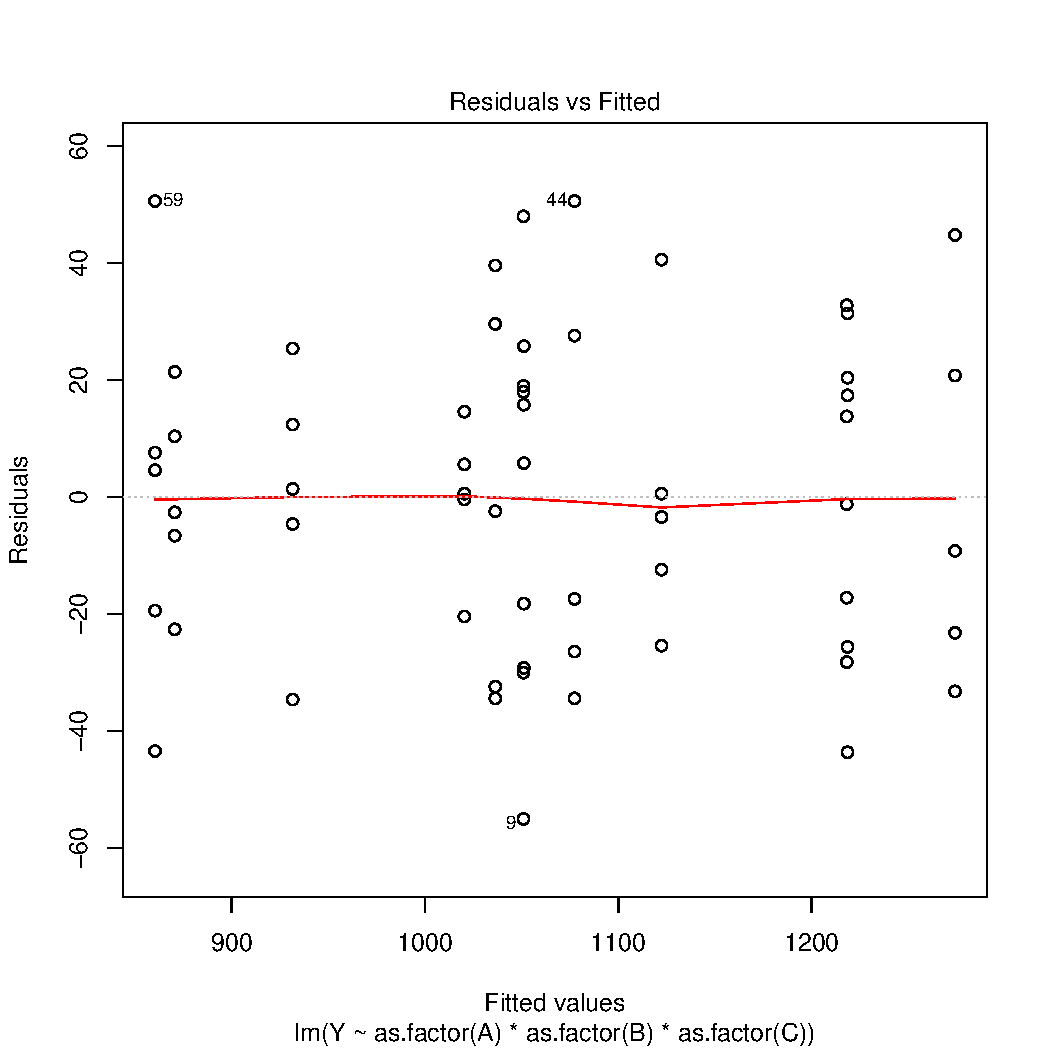
\includegraphics[width=\maxwidth]{figure/unnamed-chunk-1-1} 

\end{knitrout}

\qquad The residuals versus fitted values plots shows no sign for unequal variance.

\item

\begin{knitrout}
\definecolor{shadecolor}{rgb}{0.969, 0.969, 0.969}\color{fgcolor}\begin{kframe}
\begin{alltt}
  \hlkwd{plot}\hlstd{(fit,} \hlkwc{which} \hlstd{=} \hlnum{2}\hlstd{)}
\end{alltt}
\end{kframe}
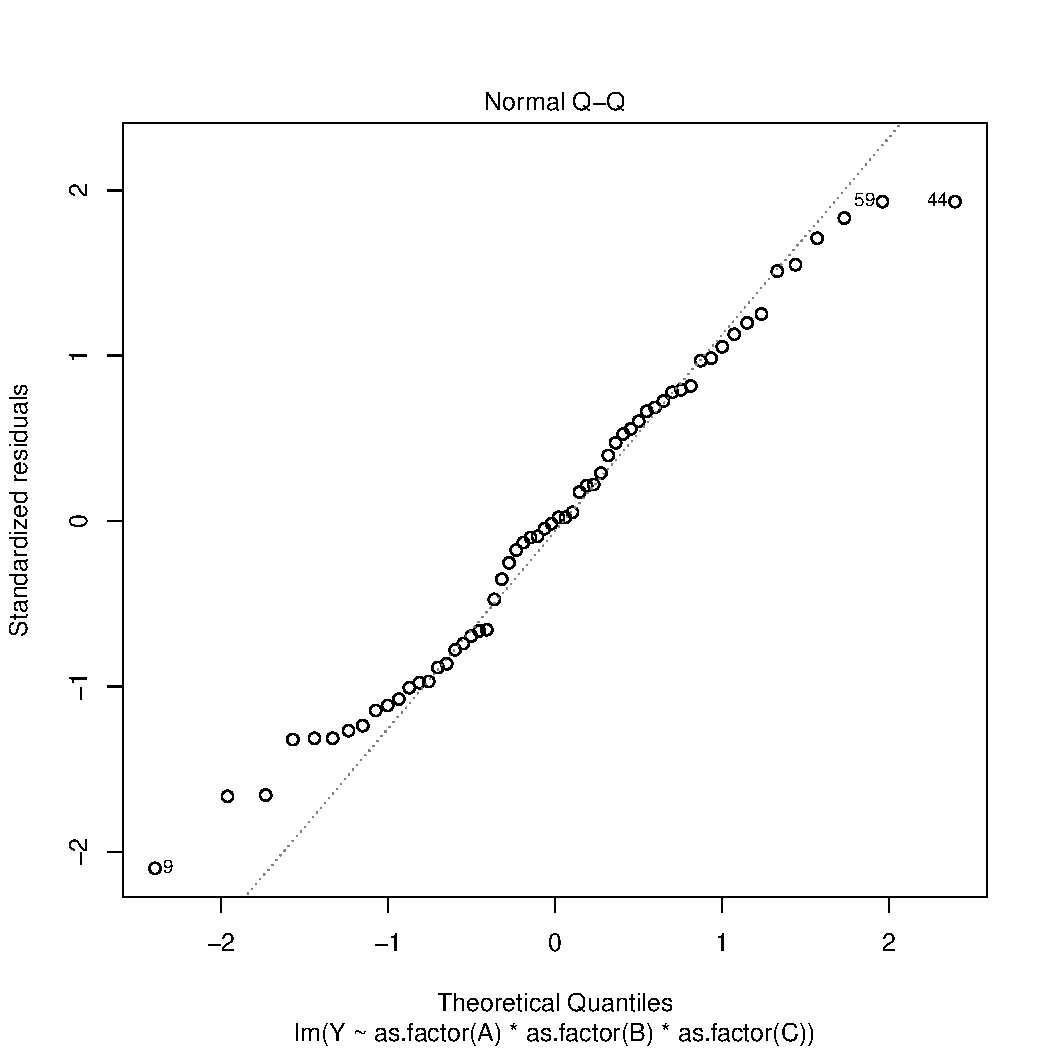
\includegraphics[width=\maxwidth]{figure/unnamed-chunk-2-1} 
\begin{kframe}\begin{alltt}
  \hlkwd{cor}\hlstd{(}\hlkwd{sort}\hlstd{(res),} \hlkwd{ppoints}\hlstd{(res))}
\end{alltt}
\begin{verbatim}
## [1] 0.9930971
\end{verbatim}
\end{kframe}
\end{knitrout}

\qquad The normal QQ plot and correlation indicates approximately normal distribution of residuals with slight light tail, so that the normality assumption seems to be reasonable here.

\end{enumerate}

\section{24.13}

\begin{enumerate}[(a)]

\item

$\bar{Y}_{ijk\cdot}$ are as follow:

\begin{knitrout}
\definecolor{shadecolor}{rgb}{0.969, 0.969, 0.969}\color{fgcolor}\begin{kframe}
\begin{alltt}
  \hlstd{means} \hlkwb{=} \hlkwd{sapply}\hlstd{(}\hlkwd{with}\hlstd{(elec,} \hlkwd{split}\hlstd{(Y,}\hlkwd{list}\hlstd{(A,B,C))), mean)}
  \hlstd{means}
\end{alltt}
\begin{verbatim}
##  1.1.1  2.1.1  1.2.1  2.2.1  1.3.1  2.3.1  1.1.2  2.1.2  1.2.2  2.2.2 
## 1218.6 1036.4 1274.2 1077.4 1218.2 1020.4 1051.0  870.6 1122.4  931.6 
##  1.3.2  2.3.2 
## 1051.2  860.4
\end{verbatim}
\end{kframe}
\end{knitrout}

\begin{knitrout}
\definecolor{shadecolor}{rgb}{0.969, 0.969, 0.969}\color{fgcolor}\begin{kframe}
\begin{alltt}
  \hlstd{elec.C} \hlkwb{=} \hlkwd{split}\hlstd{(elec, elec}\hlopt{$}\hlstd{C)}
  \hlkwd{par}\hlstd{(}\hlkwc{mfrow} \hlstd{=} \hlkwd{c}\hlstd{(}\hlnum{1}\hlstd{,}\hlnum{2}\hlstd{))}
  \hlkwd{with}\hlstd{(elec.C}\hlopt{$}\hlstr{'1'}\hlstd{,} \hlkwd{interaction.plot}\hlstd{(A, B, Y))}
  \hlkwd{with}\hlstd{(elec.C}\hlopt{$}\hlstr{'2'}\hlstd{,} \hlkwd{interaction.plot}\hlstd{(A, B, Y))}
\end{alltt}
\end{kframe}
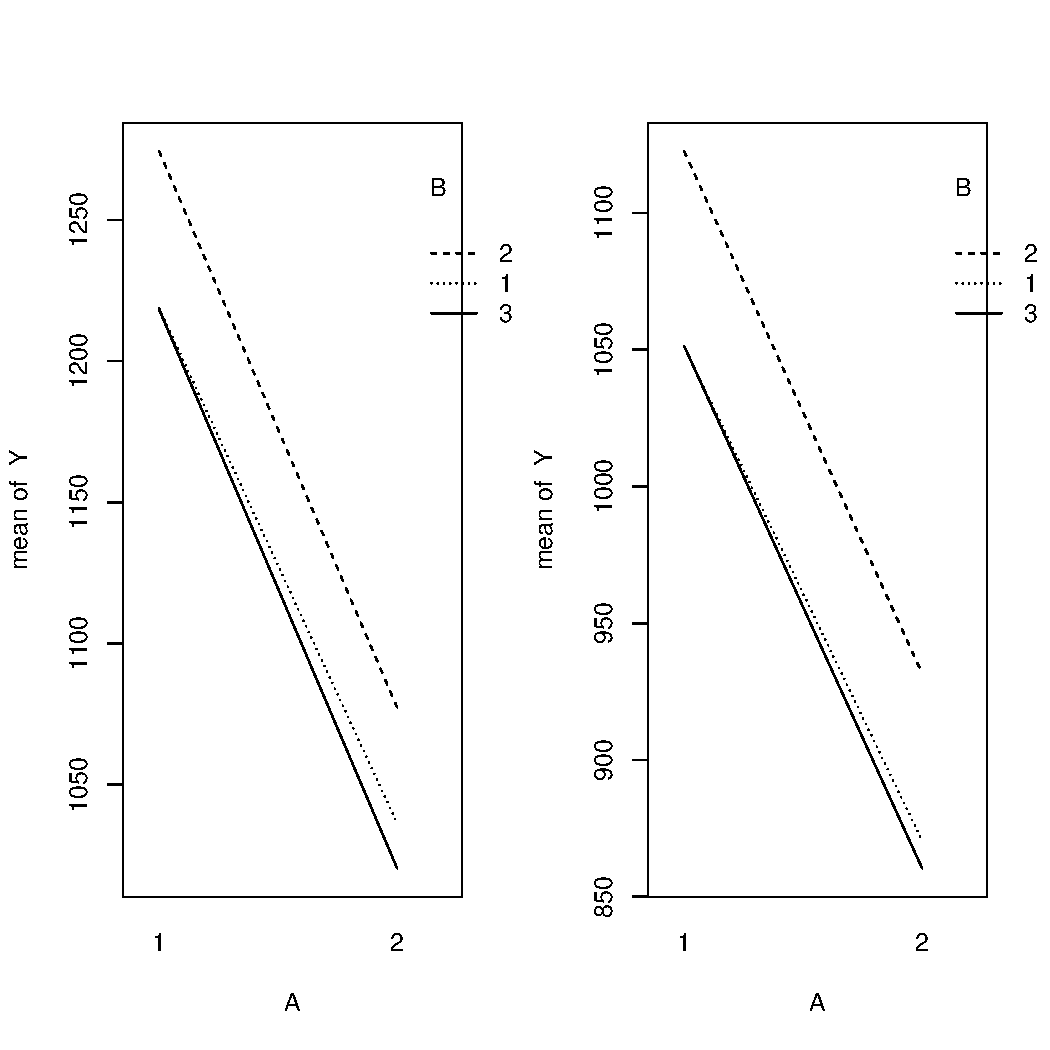
\includegraphics[width=\maxwidth]{figure/unnamed-chunk-4-1} 

\end{knitrout}

\qquad From AB plots of the estimated treatment means, the AB curves seem to be parallel, which means there's no interaction between AB, moreover, main effect A and main effect B are present.

\item

\begin{knitrout}
\definecolor{shadecolor}{rgb}{0.969, 0.969, 0.969}\color{fgcolor}\begin{kframe}
\begin{alltt}
  \hlkwd{anova}\hlstd{(fit)}
\end{alltt}
\begin{verbatim}
## Analysis of Variance Table
## 
## Response: Y
##                                        Df Sum Sq Mean Sq  F value
## as.factor(A)                            1 540361  540361 629.7603
## as.factor(B)                            2  49320   24660  28.7396
## as.factor(C)                            1 382402  382402 445.6679
## as.factor(A):as.factor(B)               2    543     271   0.3161
## as.factor(A):as.factor(C)               1     91      91   0.1064
## as.factor(B):as.factor(C)               2    911     456   0.5310
## as.factor(A):as.factor(B):as.factor(C)  2     19      10   0.0111
## Residuals                              48  41186     858         
##                                           Pr(>F)    
## as.factor(A)                           < 2.2e-16 ***
## as.factor(B)                            6.22e-09 ***
## as.factor(C)                           < 2.2e-16 ***
## as.factor(A):as.factor(B)                 0.7305    
## as.factor(A):as.factor(C)                 0.7457    
## as.factor(B):as.factor(C)                 0.5914    
## as.factor(A):as.factor(B):as.factor(C)    0.9890    
## Residuals                                           
## ---
## Signif. codes:  0 '***' 0.001 '**' 0.01 '*' 0.05 '.' 0.1 ' ' 1
\end{verbatim}
\end{kframe}
\end{knitrout}

\item

For three-factor interaction:

\begin{center}
$H_0$:all $(\alpha\beta\gamma)_{ijk}$=0

VS. $H_1$:not all $(\alpha\beta\gamma)_{ijk}$ = 0

$F^*=\frac{MSABC}{MSE} = 0.0111$

we can reject $H_0$ if $F^* > F(1-0.05;2,48)=3.19$,otherwise reject$H_1$

reject $H_1$ because $F^*<F(1-0.05;2,48)=3.19$,

therefore,we conclude $H_0$ at 0.05 level, and there's no three-factor interaction effect, and P-value = 0.9890
\end{center}

\item

For AB interaction:

\begin{center}
$H_0$:all $(\alpha\beta)_{ij}$=0

VS. $H_1$:not all $(\alpha\beta)_{ij}$ = 0

$F^*=\frac{MSAB}{MSE} = 0.3161$

we can reject $H_0$ if $F^* > F(1-0.05;2,48)=3.19$,otherwise reject$H_1$

reject $H_1$ because $F^*<F(1-0.05;2,48)=3.19$,

therefore,we conclude $H_0$ at 0.05 level, and there's no AB interaction effect, and P-value = 0.7305
\end{center}

For AC interaction:

\begin{center}
$H_0$:all $(\alpha\gamma)_{ik}$=0

VS. $H_1$:not all $(\alpha\gamma)_{ik}$ = 0

$F^*=\frac{MSAC}{MSE} = 0.1064$

we can reject $H_0$ if $F^* > F(1-0.05;1,48)=4.04$,otherwise reject$H_1$

reject $H_1$ because $F^*<F(1-0.05;2,48)=4.04$,

therefore,we conclude $H_0$ at 0.05 level, and there's no AC interaction effect, and P-value = 0.7457
\end{center}

For BC interaction:

\begin{center}
$H_0$:all $(\beta\gamma)_{jk}$=0

VS. $H_1$:not all $(\beta\gamma)_{jk}$ = 0

$F^*=\frac{MSBC}{MSE} = 0.5310$

we can reject $H_0$ if $F^* > F(1-0.05;2,48)=3.19$,otherwise reject$H_1$

reject $H_1$ because $F^*<F(1-0.05;2,48)=3.19$,

therefore,we conclude $H_0$ at 0.05 level, and there's no BC interaction effect, and P-value = 0.5914
\end{center}

\item

For A main effect:

\begin{center}
$H_0$:all $(\alpha)_{i}$=0

VS. $H_1$:not all $(\alpha)_{i}$ = 0

$F^*=\frac{MSA}{MSE} = 629.7603$

we can reject $H_0$ if $F^* > F(1-0.05;2,48)=4.04$,otherwise reject$H_1$

reject $H_0$ because $F^*>F(1-0.05;2,48)=4.04$,

therefore,we conclude $H_1$ at 0.05 level, and there's A main effect, and P-value = 2.2e-16
\end{center}

For B main effect:

\begin{center}
$H_0$:all $(\beta)_{j}$=0

VS. $H_1$:not all $(\beta)_{j}$ = 0

$F^*=\frac{MSB}{MSE} = 28.7396$

we can reject $H_0$ if $F^* > F(1-0.05;2,48)=3.19$,otherwise reject$H_1$

reject $H_0$ because $F^*>F(1-0.05;2,48)=3.19$,

therefore,we conclude $H_1$ at 0.05 level, and there's B main effect, and P-value = 6.22e-09
\end{center}

For C main effect:

\begin{center}
$H_0$:all $(\gamma)_{k}$=0

VS. $H_1$:not all $(\gamma)_{k}$ = 0

$F^*=\frac{MSC}{MSE} = 445.6679$

we can reject $H_0$ if $F^* > F(1-0.05;2,48)=4.04$,otherwise reject$H_1$

reject $H_0$ because $F^*>F(1-0.05;2,48)=3.19$,

therefore,we conclude $H_1$ at 0.05 level, and there's C main effect, and P-value = 2.2e-16
\end{center}

\item

\qquad A,B and C main effects are present, but there's no any interaction effect. As for upper bound for the family level of significance, using kimball inequality,$\alpha < 1-(1-\alpha_1)(1-\alpha_2) \cdots (1-\alpha_7)=1-(1-0.05)^7=0.3016627$

\item 

\qquad The results in part(f) confirm my graphic analysis in part(a)

\end{enumerate}

\section{24.14}

\begin{enumerate}[(a)]

\item

\begin{knitrout}
\definecolor{shadecolor}{rgb}{0.969, 0.969, 0.969}\color{fgcolor}\begin{kframe}
\begin{alltt}
  \hlstd{means} \hlkwb{=} \hlkwd{with}\hlstd{(elec,} \hlkwd{sapply}\hlstd{(}\hlkwd{list}\hlstd{(A, B, C),} \hlkwa{function}\hlstd{(}\hlkwc{x}\hlstd{)} \hlkwd{by}\hlstd{(Y, x, mean)))}
  \hlstd{means}
\end{alltt}
\begin{verbatim}
## [[1]]
## x: 1
## [1] 1155.933
## -------------------------------------------------------- 
## x: 2
## [1] 966.1333
## 
## [[2]]
## x: 1
## [1] 1044.15
## -------------------------------------------------------- 
## x: 2
## [1] 1101.4
## -------------------------------------------------------- 
## x: 3
## [1] 1037.55
## 
## [[3]]
## x: 1
## [1] 1140.867
## -------------------------------------------------------- 
## x: 2
## [1] 981.2
\end{verbatim}
\begin{alltt}
  \hlstd{D1.hat} \hlkwb{=} \hlstd{means[[}\hlnum{1}\hlstd{]][}\hlnum{1}\hlstd{]} \hlopt{-} \hlstd{means[[}\hlnum{1}\hlstd{]][}\hlnum{2}\hlstd{]}
  \hlstd{D2.hat} \hlkwb{=} \hlstd{means[[}\hlnum{2}\hlstd{]][}\hlnum{1}\hlstd{]} \hlopt{-} \hlstd{means[[}\hlnum{2}\hlstd{]][}\hlnum{2}\hlstd{]}
  \hlstd{D3.hat} \hlkwb{=} \hlstd{means[[}\hlnum{2}\hlstd{]][}\hlnum{1}\hlstd{]} \hlopt{-} \hlstd{means[[}\hlnum{2}\hlstd{]][}\hlnum{3}\hlstd{]}
  \hlstd{D4.hat} \hlkwb{=} \hlstd{means[[}\hlnum{2}\hlstd{]][}\hlnum{2}\hlstd{]} \hlopt{-} \hlstd{means[[}\hlnum{2}\hlstd{]][}\hlnum{3}\hlstd{]}
  \hlstd{D5.hat} \hlkwb{=} \hlstd{means[[}\hlnum{3}\hlstd{]][}\hlnum{1}\hlstd{]} \hlopt{-} \hlstd{means[[}\hlnum{3}\hlstd{]][}\hlnum{2}\hlstd{]}
  \hlstd{mse} \hlkwb{=} \hlkwd{anova}\hlstd{(fit)[}\hlstr{"Residuals"}\hlstd{,} \hlnum{3}\hlstd{]}
  \hlstd{S_D1} \hlkwb{=} \hlkwd{sqrt}\hlstd{(mse}\hlopt{/}\hlstd{(n}\hlopt{*}\hlstd{b}\hlopt{*}\hlstd{c)}\hlopt{*}\hlnum{2}\hlstd{)}
  \hlstd{S_D2} \hlkwb{=} \hlkwd{sqrt}\hlstd{(mse}\hlopt{/}\hlstd{(n}\hlopt{*}\hlstd{a}\hlopt{*}\hlstd{c)}\hlopt{*}\hlnum{2}\hlstd{)}
  \hlstd{S_D3} \hlkwb{=} \hlkwd{sqrt}\hlstd{(mse}\hlopt{/}\hlstd{(n}\hlopt{*}\hlstd{a}\hlopt{*}\hlstd{c)}\hlopt{*}\hlnum{2}\hlstd{)}
  \hlstd{S_D4} \hlkwb{=} \hlkwd{sqrt}\hlstd{(mse}\hlopt{/}\hlstd{(n}\hlopt{*}\hlstd{a}\hlopt{*}\hlstd{c)}\hlopt{*}\hlnum{2}\hlstd{)}
  \hlstd{S_D5} \hlkwb{=} \hlkwd{sqrt}\hlstd{(mse}\hlopt{/}\hlstd{(n}\hlopt{*}\hlstd{a}\hlopt{*}\hlstd{b)}\hlopt{*}\hlnum{2}\hlstd{)}
  \hlstd{B} \hlkwb{=} \hlkwd{qt}\hlstd{(}\hlnum{1}\hlopt{-}\hlnum{.1}\hlopt{/}\hlstd{(}\hlnum{2}\hlopt{*}\hlnum{5}\hlstd{),} \hlnum{48}\hlstd{)}
  \hlkwd{c}\hlstd{(D1.hat}\hlopt{-}\hlstd{B}\hlopt{*}\hlstd{S_D1, D1.hat}\hlopt{+}\hlstd{B}\hlopt{*}\hlstd{S_D1)}
\end{alltt}
\begin{verbatim}
##        1        1 
## 171.5984 208.0016
\end{verbatim}
\begin{alltt}
  \hlkwd{c}\hlstd{(D2.hat}\hlopt{-}\hlstd{B}\hlopt{*}\hlstd{S_D2, D2.hat}\hlopt{+}\hlstd{B}\hlopt{*}\hlstd{S_D2)}
\end{alltt}
\begin{verbatim}
##         1         1 
## -79.54229 -34.95771
\end{verbatim}
\begin{alltt}
  \hlkwd{c}\hlstd{(D3.hat}\hlopt{-}\hlstd{B}\hlopt{*}\hlstd{S_D3, D3.hat}\hlopt{+}\hlstd{B}\hlopt{*}\hlstd{S_D3)}
\end{alltt}
\begin{verbatim}
##         1         1 
## -15.69229  28.89229
\end{verbatim}
\begin{alltt}
  \hlkwd{c}\hlstd{(D4.hat}\hlopt{-}\hlstd{B}\hlopt{*}\hlstd{S_D4, D4.hat}\hlopt{+}\hlstd{B}\hlopt{*}\hlstd{S_D4)}
\end{alltt}
\begin{verbatim}
##        2        2 
## 41.55771 86.14229
\end{verbatim}
\begin{alltt}
  \hlkwd{c}\hlstd{(D5.hat}\hlopt{-}\hlstd{B}\hlopt{*}\hlstd{S_D5, D5.hat}\hlopt{+}\hlstd{B}\hlopt{*}\hlstd{S_D5)}
\end{alltt}
\begin{verbatim}
##        1        1 
## 141.4651 177.8682
\end{verbatim}
\end{kframe}
\end{knitrout}

\begin{center}
171.5984 $\leq D_1 \leq  $208.0016 \\
-79.54229 $\leq D_2 \leq  $-34.95771 \\
-15.69229 $\leq D_3 \leq  $28.89229 \\
41.55771 $\leq D_4 \leq  $86.14229 \\
141.4651 $\leq D_5 \leq  $177.8682 \\
\end{center}

\item

\begin{knitrout}
\definecolor{shadecolor}{rgb}{0.969, 0.969, 0.969}\color{fgcolor}\begin{kframe}
\begin{alltt}
\hlstd{dat.231} \hlkwb{=} \hlstd{elec[}\hlkwd{with}\hlstd{(elec, A} \hlopt{==} \hlnum{2} \hlopt{&} \hlstd{B} \hlopt{==} \hlnum{3} \hlopt{&} \hlstd{C} \hlopt{==} \hlnum{1}\hlstd{), ]}
\hlstd{means} \hlkwb{=} \hlkwd{mean}\hlstd{(dat.231}\hlopt{$}\hlstd{Y)}
\hlstd{s} \hlkwb{=} \hlkwd{sqrt}\hlstd{(mse}\hlopt{/}\hlstd{n)}
\hlstd{t.} \hlkwb{=} \hlkwd{qt}\hlstd{(}\hlnum{1} \hlopt{-} \hlnum{.05}\hlopt{/}\hlnum{2}\hlstd{, (n} \hlopt{-} \hlnum{1}\hlstd{)}\hlopt{*}\hlstd{a}\hlopt{*}\hlstd{b}\hlopt{*}\hlstd{c)}
\hlkwd{c}\hlstd{(means} \hlopt{-} \hlstd{t.}\hlopt{*}\hlstd{s, means} \hlopt{+} \hlstd{t.}\hlopt{*}\hlstd{s)}
\end{alltt}
\begin{verbatim}
## [1]  994.0608 1046.7392
\end{verbatim}
\end{kframe}
\end{knitrout}

\qquad Therefore,$\mu_{231}$ with a 95 percent confidence interval is 994.0608 $\leq \mu_{231} \leq  $ 1046.7392

\end{enumerate}

\section{24.16}

\begin{enumerate}[(a)]

\item

\begin{knitrout}
\definecolor{shadecolor}{rgb}{0.969, 0.969, 0.969}\color{fgcolor}\begin{kframe}
\begin{alltt}
  \hlstd{dat.reg} \hlkwb{=} \hlstd{elec[}\hlopt{-}\hlkwd{c}\hlstd{(}\hlnum{19}\hlstd{,} \hlnum{40}\hlstd{,} \hlnum{43}\hlstd{), ]}
  \hlstd{x1} \hlkwb{=} \hlstd{dat.reg}\hlopt{$}\hlstd{A}
  \hlstd{x1} \hlkwb{=} \hlkwd{replace}\hlstd{(x1,} \hlkwd{which}\hlstd{(dat.reg}\hlopt{$}\hlstd{A} \hlopt{==} \hlnum{2}\hlstd{),} \hlopt{-}\hlnum{1}\hlstd{)}
  \hlstd{x2} \hlkwb{=} \hlstd{dat.reg}\hlopt{$}\hlstd{B}
  \hlstd{x2} \hlkwb{=} \hlkwd{replace}\hlstd{(x2,} \hlkwd{which}\hlstd{(dat.reg}\hlopt{$}\hlstd{B} \hlopt{==} \hlnum{3}\hlstd{),} \hlopt{-}\hlnum{1}\hlstd{)}
  \hlstd{x2} \hlkwb{=} \hlkwd{replace}\hlstd{(x2,} \hlkwd{which}\hlstd{(dat.reg}\hlopt{$}\hlstd{B} \hlopt{==} \hlnum{2}\hlstd{),} \hlnum{0}\hlstd{)}
  \hlstd{x3} \hlkwb{=} \hlstd{dat.reg}\hlopt{$}\hlstd{B}
  \hlstd{x3} \hlkwb{=} \hlkwd{replace}\hlstd{(x3,} \hlkwd{which}\hlstd{(dat.reg}\hlopt{$}\hlstd{B} \hlopt{==} \hlnum{3}\hlstd{),} \hlopt{-}\hlnum{1}\hlstd{)}
  \hlstd{x3} \hlkwb{=} \hlkwd{replace}\hlstd{(x3,} \hlkwd{which}\hlstd{(dat.reg}\hlopt{$}\hlstd{B} \hlopt{==} \hlnum{1}\hlstd{),} \hlnum{0}\hlstd{)}
  \hlstd{x3} \hlkwb{=} \hlkwd{replace}\hlstd{(x3,} \hlkwd{which}\hlstd{(dat.reg}\hlopt{$}\hlstd{B} \hlopt{==} \hlnum{2}\hlstd{),} \hlnum{1}\hlstd{)}
  \hlstd{x4} \hlkwb{=} \hlstd{dat.reg}\hlopt{$}\hlstd{C}
  \hlstd{x4} \hlkwb{=} \hlkwd{replace}\hlstd{(x4,} \hlkwd{which}\hlstd{(dat.reg}\hlopt{$}\hlstd{C} \hlopt{==} \hlnum{2}\hlstd{),} \hlopt{-}\hlnum{1}\hlstd{)}
  \hlstd{model.full} \hlkwb{=} \hlkwd{lm}\hlstd{(dat.reg}\hlopt{$}\hlstd{Y} \hlopt{~} \hlstd{x1}\hlopt{*}\hlstd{(x2}\hlopt{+}\hlstd{x3)}\hlopt{*}\hlstd{x4)}
  \hlstd{sse.full} \hlkwb{=} \hlkwd{sum}\hlstd{(}\hlkwd{resid}\hlstd{(model.full)}\hlopt{^}\hlnum{2}\hlstd{)}
\end{alltt}
\end{kframe}
\end{knitrout}

For full model:
\begin{displaymath}
\begin{split}
Y_{ijkm} &= \mu_{\cdots} + \alpha_1 X_{ijkm1} +  \beta_1 X_{ijkm2} + \beta_2 X_{ijkm3} +\gamma X_{ijkm4}\\
         &+ (\alpha\beta)_{11} X_{ijkm1} X_{ijkm2} + (\alpha\beta)_{12} X_{ijkm1} X_{ijkm3} +(\alpha\gamma)_{11} X_{ijkm1} X_{ijkm4} \\
         &+ (\beta\gamma)_{11} X_{ijkm2} X_{ijkm4} + (\beta\gamma)_{21} X_{ijkm3} X_{ijkm4} +(\alpha\beta\gamma)_{111} X_{ijkm1} X_{ijkm2} X_{ijkm4} \\
         &+ (\alpha\beta\gamma)_{121} X_{ijkm1} X_{ijkm3} X_{ijkm4} + \epsilon_{ijkm}
\end{split}
\end{displaymath}

\begin{eqnarray}
X_{ijkm1} =
\begin{cases}
1       & \text{if factor A is level 1} \\
-1   & \text{if factor A is level 2}
\end{cases}
\end{eqnarray}

\begin{eqnarray}
X_{ijkm2} =
\begin{cases}
1       & \text{if factor B is level 1} \\
-1   & \text{if factor B is level 3} \\
0 & else
\end{cases}
\end{eqnarray}

\begin{eqnarray}
X_{ijkm3} =
\begin{cases}
1       & \text{if factor B is level 2} \\
-1   & \text{if factor B is level 3} \\
0 & else
\end{cases}
\end{eqnarray}

\begin{eqnarray}
X_{ijkm4} =
\begin{cases}
1       & \text{if factor C is level 1} \\
-1   & \text{if factor C is level 2}
\end{cases}
\end{eqnarray}

\item

\begin{knitrout}
\definecolor{shadecolor}{rgb}{0.969, 0.969, 0.969}\color{fgcolor}\begin{kframe}
\begin{alltt}
  \hlstd{model.red} \hlkwb{=} \hlkwd{lm}\hlstd{(dat.reg}\hlopt{$}\hlstd{Y} \hlopt{~} \hlstd{x1}\hlopt{*}\hlstd{(x2}\hlopt{+}\hlstd{x3)}\hlopt{*}\hlstd{x4} \hlopt{-}\hlstd{x4)}
  \hlstd{sse.red} \hlkwb{=} \hlkwd{sum}\hlstd{(}\hlkwd{resid}\hlstd{(model.red)}\hlopt{^}\hlnum{2}\hlstd{)}
\end{alltt}
\end{kframe}
\end{knitrout}

For reduced model:
\begin{displaymath}
\begin{split}
Y_{ijkm} &= \mu_{\cdots} + \alpha_1 X_{ijkm1} +  \beta_1 X_{ijkm2} + \beta_2 X_{ijkm3} \\
         &+ (\alpha\beta)_{11} X_{ijkm1} X_{ijkm2} + (\alpha\beta)_{12} X_{ijkm1} X_{ijkm3} +(\alpha\gamma)_{11} X_{ijkm1} X_{ijkm4} \\
         &+ (\beta\gamma)_{11} X_{ijkm2} X_{ijkm4} + (\beta\gamma)_{21} X_{ijkm3} X_{ijkm4} +(\alpha\beta\gamma)_{111} X_{ijkm1} X_{ijkm2} X_{ijkm4} \\
         &+ (\alpha\beta\gamma)_{121} X_{ijkm1} X_{ijkm3} X_{ijkm4} + \epsilon_{ijkm}
\end{split}
\end{displaymath}

\item

\begin{knitrout}
\definecolor{shadecolor}{rgb}{0.969, 0.969, 0.969}\color{fgcolor}\begin{kframe}
\begin{alltt}
  \hlkwd{summary}\hlstd{(model.full)}
\end{alltt}
\begin{verbatim}
## 
## Call:
## lm(formula = dat.reg$Y ~ x1 * (x2 + x3) * x4)
## 
## Residuals:
##    Min     1Q Median     3Q    Max 
##  -55.0  -23.2    0.6   20.4   50.6 
## 
## Coefficients:
##              Estimate Std. Error t value Pr(>|t|)    
## (Intercept) 1062.1667     3.9426 269.409  < 2e-16 ***
## x1            94.8250     3.9426  24.052  < 2e-16 ***
## x2           -17.8542     5.5757  -3.202   0.0025 ** 
## x3            42.4708     5.6571   7.508 1.81e-09 ***
## x4            79.8000     3.9426  20.241  < 2e-16 ***
## x1:x2         -4.3375     5.5757  -0.778   0.4407    
## x1:x3          2.0125     5.6571   0.356   0.7237    
## x1:x4          0.2083     3.9426   0.053   0.9581    
## x2:x4          3.3875     5.5757   0.608   0.5465    
## x3:x4         -5.3375     5.6571  -0.944   0.3505    
## x1:x2:x4       0.4042     5.5757   0.072   0.9425    
## x1:x3:x4      -1.9458     5.6571  -0.344   0.7325    
## ---
## Signif. codes:  0 '***' 0.001 '**' 0.01 '*' 0.05 '.' 0.1 ' ' 1
## 
## Residual standard error: 29.63 on 45 degrees of freedom
## Multiple R-squared:  0.9595,	Adjusted R-squared:  0.9496 
## F-statistic: 96.96 on 11 and 45 DF,  p-value: < 2.2e-16
\end{verbatim}
\begin{alltt}
  \hlkwd{summary}\hlstd{(model.red)}
\end{alltt}
\begin{verbatim}
## 
## Call:
## lm(formula = dat.reg$Y ~ x1 * (x2 + x3) * x4 - x4)
## 
## Residuals:
##     Min      1Q  Median      3Q     Max 
## -130.11  -73.71   31.51   74.71  137.88 
## 
## Coefficients:
##             Estimate Std. Error t value Pr(>|t|)    
## (Intercept) 1063.731     12.393  85.834  < 2e-16 ***
## x1            96.390     12.393   7.778  6.3e-10 ***
## x2           -14.725     17.523  -0.840    0.405    
## x3            40.906     17.784   2.300    0.026 *  
## x1:x2        -10.596     17.503  -0.605    0.548    
## x1:x3          9.836     17.744   0.554    0.582    
## x1:x4          1.773     12.393   0.143    0.887    
## x2:x4          3.388     17.529   0.193    0.848    
## x3:x4        -10.032     17.770  -0.565    0.575    
## x1:x2:x4       3.534     17.523   0.202    0.841    
## x1:x3:x4      -3.511     17.784  -0.197    0.844    
## ---
## Signif. codes:  0 '***' 0.001 '**' 0.01 '*' 0.05 '.' 0.1 ' ' 1
## 
## Residual standard error: 93.15 on 46 degrees of freedom
## Multiple R-squared:  0.5909,	Adjusted R-squared:  0.502 
## F-statistic: 6.645 on 10 and 46 DF,  p-value: 2.836e-06
\end{verbatim}
\begin{alltt}
  \hlstd{sse.full}
\end{alltt}
\begin{verbatim}
## [1] 39499.9
\end{verbatim}
\begin{alltt}
  \hlstd{sse.red}
\end{alltt}
\begin{verbatim}
## [1] 399106.9
\end{verbatim}
\end{kframe}
\end{knitrout}

SSE(F)=39499.9, df(F)=45

SSE(R)=399106.9, df(R)=46

\begin{center}
$H_0$:all $(\gamma)_{1}$=0

VS. $H_1$:not all $(\gamma)_{1}$ = 0

$F^*=\frac{(SSE(R)-SSE(F))/(df(R)-df(F))}{SSE(F)/df(F)} = \frac{359607/1}{39499.9/45} = 409.6799$

we can reject $H_0$ if $F^* > F(1-0.05;1,45)=4.056612$,otherwise reject$H_1$

reject $H_0$ because $F^*>F(1-0.05;1,45)=3.19$,

therefore,we conclude $H_1$ at 0.05 level, and there's C main effect, and P-value is 3.114909e-24, very close to zero.
\end{center}

\begin{knitrout}
\definecolor{shadecolor}{rgb}{0.969, 0.969, 0.969}\color{fgcolor}\begin{kframe}
\begin{alltt}
  \hlstd{f.star} \hlkwb{=} \hlstd{(sse.red} \hlopt{-} \hlstd{sse.full)} \hlopt{/} \hlstd{(sse.full}\hlopt{/}\hlnum{45}\hlstd{)}
  \hlkwd{qf}\hlstd{(}\hlnum{1} \hlopt{-} \hlnum{.05}\hlstd{,} \hlnum{1}\hlstd{,} \hlnum{45}\hlstd{)}
\end{alltt}
\begin{verbatim}
## [1] 4.056612
\end{verbatim}
\begin{alltt}
  \hlkwd{pf}\hlstd{(f.star,} \hlnum{1}\hlstd{,} \hlnum{45}\hlstd{,} \hlkwc{lower} \hlstd{=} \hlnum{FALSE}\hlstd{)}
\end{alltt}
\begin{verbatim}
## [1] 3.114909e-24
\end{verbatim}
\end{kframe}
\end{knitrout}

\item

\begin{knitrout}
\definecolor{shadecolor}{rgb}{0.969, 0.969, 0.969}\color{fgcolor}\begin{kframe}
\begin{alltt}
  \hlstd{D.hat} \hlkwb{=} \hlnum{159.6}
  \hlstd{n.s} \hlkwb{=} \hlkwd{with}\hlstd{(dat.reg,} \hlkwd{by}\hlstd{(Y,} \hlkwd{list}\hlstd{(A, B, C), length))}
  \hlstd{s} \hlkwb{=} \hlkwd{sqrt}\hlstd{(sse.full}\hlopt{/}\hlstd{(}\hlkwd{nrow}\hlstd{(dat.reg)} \hlopt{-} \hlstd{a}\hlopt{*}\hlstd{b}\hlopt{*}\hlstd{c)} \hlopt{/} \hlstd{(a}\hlopt{^}\hlnum{2}\hlopt{*}\hlstd{b}\hlopt{^}\hlnum{2}\hlstd{)} \hlopt{*} \hlkwd{sum}\hlstd{(}\hlnum{1}\hlopt{/}\hlstd{n.s))}
  \hlstd{s}
\end{alltt}
\begin{verbatim}
## [1] 7.885161
\end{verbatim}
\begin{alltt}
  \hlstd{t.} \hlkwb{=} \hlkwd{qt}\hlstd{(}\hlnum{1} \hlopt{-} \hlnum{.05}\hlopt{/}\hlnum{2}\hlstd{,} \hlkwd{nrow}\hlstd{(dat.reg)} \hlopt{-} \hlstd{a}\hlopt{*}\hlstd{b}\hlopt{*}\hlstd{c)}
  \hlkwd{c}\hlstd{(D.hat} \hlopt{-} \hlstd{s}\hlopt{*}\hlstd{t., D.hat} \hlopt{+} \hlstd{s}\hlopt{*}\hlstd{t.)}
\end{alltt}
\begin{verbatim}
## [1] 143.7185 175.4815
\end{verbatim}
\end{kframe}
\end{knitrout}

$\hat{D} = \hat{\mu}_{\cdot \cdot 1} - \hat{\mu}_{\cdot \cdot 2}= \hat{\gamma}_1 - \hat{\gamma}_2 = 2\hat{\gamma}_1=2*79.8=159.6$

MSE = $\frac{SSE(F)}{df(F)} = 877.7756$

$Var(\bar{Y}_{ijk\cdot}) = \frac{MSE}{n_{ijk}}$

$Var(\hat{\mu}_{\cdot \cdot 1}) = Var(\frac{\sum_{i=1}^a\sum_{j=1}^b \bar{Y}_{ij1\cdot}}{ab}) = \frac{MSE}{a^2b^2} \sum_{i=1}^a\sum_{j=1}^b \frac{1}{n_{ij1}}$

$S(\hat{D}) = \sqrt{Var(\hat{\mu}_{\cdot \cdot 1})+Var(\hat{\mu}_{\cdot \cdot 2})} = \sqrt{\frac{MSE}{a^2b^2} \sum_{i=1}^a\sum_{j=1}^b\sum_{k=1}^c \frac{1}{n_{ijk}}} = 7.885161$

t = t(1- 0.05/2; 45) = 2.014103

Therefore,$\hat{D} \pm S(\hat{D})*t$, which means 143.7185 $\leq D \leq$ 175.4815

\end{enumerate}

\section{24.18}

\begin{knitrout}
\definecolor{shadecolor}{rgb}{0.969, 0.969, 0.969}\color{fgcolor}\begin{kframe}
\begin{alltt}
  \hlstd{n} \hlkwb{=} \hlnum{5}
  \hlstd{s} \hlkwb{=} \hlkwd{sqrt}\hlstd{(}\hlnum{29}\hlopt{^}\hlnum{2}\hlopt{/}\hlstd{(n}\hlopt{*}\hlstd{b}\hlopt{*}\hlstd{c)}\hlopt{*}\hlnum{2}\hlstd{)}
  \hlstd{B} \hlkwb{=} \hlkwd{qt}\hlstd{(}\hlnum{1} \hlopt{-} \hlnum{.1}\hlopt{/}\hlstd{(}\hlnum{2}\hlopt{*}\hlnum{5}\hlstd{), n}\hlopt{*}\hlstd{a}\hlopt{*}\hlstd{b}\hlopt{*}\hlstd{c} \hlopt{-} \hlstd{a}\hlopt{*}\hlstd{b}\hlopt{*}\hlstd{c)}
  \hlstd{B}\hlopt{*}\hlstd{s}
\end{alltt}
\begin{verbatim}
## [1] 18.01992
\end{verbatim}
\begin{alltt}
  \hlstd{n} \hlkwb{=} \hlnum{7}
  \hlstd{s} \hlkwb{=} \hlkwd{sqrt}\hlstd{(}\hlnum{29}\hlopt{^}\hlnum{2}\hlopt{/}\hlstd{(n}\hlopt{*}\hlstd{a}\hlopt{*}\hlstd{c)}\hlopt{*}\hlnum{2}\hlstd{)}
  \hlstd{B} \hlkwb{=} \hlkwd{qt}\hlstd{(}\hlnum{1} \hlopt{-} \hlnum{.1}\hlopt{/}\hlstd{(}\hlnum{2}\hlopt{*}\hlnum{5}\hlstd{), n}\hlopt{*}\hlstd{a}\hlopt{*}\hlstd{b}\hlopt{*}\hlstd{c} \hlopt{-} \hlstd{a}\hlopt{*}\hlstd{b}\hlopt{*}\hlstd{c)}
  \hlstd{B}\hlopt{*}\hlstd{s}
\end{alltt}
\begin{verbatim}
## [1] 18.44065
\end{verbatim}
\begin{alltt}
  \hlstd{n} \hlkwb{=} \hlnum{5}
  \hlstd{s} \hlkwb{=} \hlkwd{sqrt}\hlstd{(}\hlnum{29}\hlopt{^}\hlnum{2}\hlopt{/}\hlstd{(n}\hlopt{*}\hlstd{a}\hlopt{*}\hlstd{b)}\hlopt{*}\hlnum{2}\hlstd{)}
  \hlstd{B} \hlkwb{=} \hlkwd{qt}\hlstd{(}\hlnum{1} \hlopt{-} \hlnum{.1}\hlopt{/}\hlstd{(}\hlnum{2}\hlopt{*}\hlnum{5}\hlstd{), n}\hlopt{*}\hlstd{a}\hlopt{*}\hlstd{b}\hlopt{*}\hlstd{c} \hlopt{-} \hlstd{a}\hlopt{*}\hlstd{b}\hlopt{*}\hlstd{c)}
  \hlstd{B}\hlopt{*}\hlstd{s}
\end{alltt}
\begin{verbatim}
## [1] 18.01992
\end{verbatim}
\end{kframe}
\end{knitrout}

\quad We find that 
  \begin{itemize}
  \item
    for $L_1$, if the precision of each of the estimates should not exceed, the smallest sample size is 5 
  \item
    for $L_2, L_3$ and $L_4$, if the precision of each of the estimates should not exceed, the smallest sample size is 7 
  \item 
    for $L_1$, if the precision of each of the estimates should not exceed, the smallest sample size is 5.
  \end{itemize}
Therefore, the required sample size should be n $\geq$ 7.

\section{24.19}

\begin{displaymath}
\begin{split}
\sum_i(\alpha\beta\gamma)_{ijk} &= \sum_i(\mu_{ijk} - \mu_{ij\cdot} - \mu_{i\cdot k} - \mu_{\cdot jk} + \mu_{i\cdot\cdot} + \mu_{\cdot j \cdot} + \mu_{\cdot \cdot k} - \mu_{\cdots}) \\
                                &= a\mu_{\cdot jk} - a\mu_{\cdot j\cdot} - a\mu_{\cdot\cdot k} - a\mu_{\cdot jk} + a\mu_{\cdot\cdot\cdot} + a\mu_{\cdot j \cdot} + a\mu_{\cdot \cdot k} - a\mu_{\cdots} \\
                                &= 0
\end{split}
\end{displaymath}

\section{24.20}

The model without three-factor interaction is:
\begin{center}
$Y_{ijk} = \mu_{\cdots} + \alpha_i + \beta_j + \gamma_k + (\alpha\beta)_{ij} + (\alpha\gamma)_{ik} + (\beta\gamma)_{jk} + \epsilon_{ijk}$
\end{center}

\begin{table}[h]
\begin{tabular}{llll}
         & SS   & d.f.            & MS   \\ \hline
A        & SSA  & a-1             & MSA  \\
B        & SSB  & b-1             & MSB  \\
C        & SSC  & c-1             & MSC  \\
AB       & SSAB & (a-1)(b-1)      & MSAB \\
AC       & SSAC & (a-1)(c-1)      & MSAC \\
BC       & SSBC & (b-1)(c-1)      & MSBC \\
         &      &                 &      \\ \hline
Residual & SSE  & (a-1)(b-1)(c-1) & MSE  \\
Total    & SSTO & abc-1           &     
\end{tabular}
\end{table}

\section{24.21}

\begin{displaymath}
\begin{split}
Var(\hat{L}) &= Var(\sum\sum c_{ij}\bar{Y}_{ij\cdot\cdot}) \\
             &= \sum\sum c_{ij}^2 Var(\bar{Y}_{ij\cdot\cdot}) \\
             &= \sum\sum c_{ij}^2 \frac{\sigma^2}{cn} \\
             &= \frac{\sigma^2}{cn} \sum\sum c_{ij}^2
\end{split}
\end{displaymath} 

\end{document}
